\documentclass[10pt]{article}
\usepackage[usenames]{color} %used for font color
\usepackage{amssymb} %maths
\usepackage{amsmath} %maths
\usepackage{graphicx}
\usepackage[utf8]{inputenc} %useful to type directly diacritic characters

\begin{document}


Hello, world!

I have to write a program based on the least-squares function : 

\begin{equation}
\chi^2 = \sum_{i=0}^{n-1} \left(\frac{(y_i - y(x_i))}{\sigma_i}\right)^2
\end{equation}

``But Sal, that's really hard, can you show me something easier?'' you say. 

``But of course, my students!''

Let's say you want to write a simple function like $y = \sin{x}$. Or, you can do easy subscripts (like $x_i$) and superscripts (like $x^2$). 

We can even speak in Greek! $\alpha\beta\gamma\delta\epsilon$ and I don't remember the rest. 

Oh! You can do sections too. As follows. 

\section{Problem 1}
\label{section1}

Problem 1 would go here. 

\section{Problem 2}

Problem 2 would go here. It comes after Section~\ref{section1}. Take a look in my Feedback, Section~\ref{feedback}. 

\section{Feedback}
\label{feedback}

This class really needs a better room, dude. 


\section{Problems I'm having}
\label{problems}

I can't get pyplot installed, wtf is going on? 



\begin{figure}[h!]
    \centering
    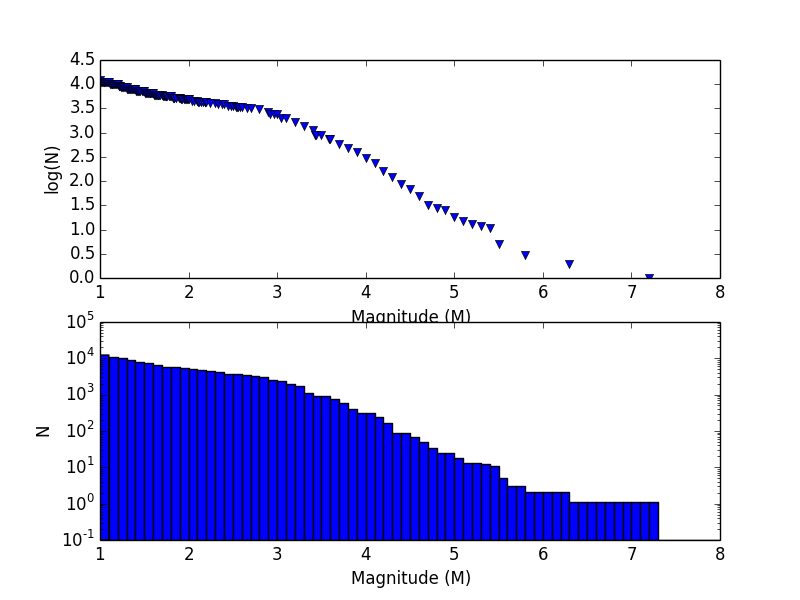
\includegraphics[width=100mm]{figure_1.png}
    \caption{\label{fig:quake}Output of quake.py }
\end{figure}


\end{document} 